\section{Auswertung}

Im folgenden lassen sich die aufgenommen Messdaten aus den Tabellen ... bis .. auswerten. Dabei wird zunächst die Grenzspannung $U_{g}$ bei den verwendeten Frequenzen des Lichts mittels linearer Regression ermittelt und es ergeben sich
die Größen $h$/$e_{0}$ sowie die materialabhängige Austrittsarbeit.

\subsection{Bestimmung der Grenzspannung}

Zunächst lassen sich für alle aufgenommenen Strom- und Spannungwerte der einzelnen Frequenzen in Abhängigkeit voneinander abbilden. Dabei gilt die Annahme \eqref{eq:whatisthis}, deshalb werden im Folgenden $\sqrt{I}$-$U$ Diagramme dargestellt.
Die Grenzspannungen ergeben sich dabei aus den Spannungwerten bei denen $\sqrt{I} = 0$ gilt.
Für eine genauere Bestimmung der Grenzspannung wird eine lineare Ausgleichsrechnung in der Nähe der Grenzspannung durchgeführt.  Dabei wurden je nach Messreihe unterschiedliche große
Intervalle linearisiert, um genauere Grenzspannungen zu erhalten. 
Die Ausgleichsgeraden wurden hier durch einen \enquote{Polyfit} in Python mit Numpy \cite{numpy} ermittelt und sind in den jeweiligen Abbildungen \ref{fig:gelb} bis \ref{fig:GIGAviolet} mit abgebildet.
\\
Die allgemeine Form der linearen Ausgleichsgeraden sieht folgendermaßen aus
\begin{equation}
    \label{eqn:okay}
y = ax + b.
\end{equation}
Die Parameter $a$ und $b$ sind in den Untertiteln der einzelnen Abbildungen \ref{fig:gelb} bis \ref{fig:GIGAviolet} angegeben.
\\
Aus den Schnittpunkten der Ausgleichsgeraden mit der Abszisse ergeben sich die in der Tabelle \ref{tab:ugrenz} angegebenen Grenzspannungen.
Diese ergeben sich durch umstellen nach $x$ der Gleichung \eqref{eqn:okay} bei $y = 0$ zu 
\begin{equation*}
U_g = -\frac{b}{a}.
\end{equation*}
Da $a$ und $b$ fehlerbehaftet sind ergeben sich Fehler auf die Grenzspannung $U_g$ durch die Gaußsche Fehlerfortpflanzung
\begin{equation*}
\increment U_g = \frac{1}{|a|} \sqrt{(\increment b)^2 + \left( \frac{b \cdot \increment a}{a}\right)^2}.
\end{equation*}
\begin{table}
    \caption{Ermittelte Grenzspannungen $\protect U_{g}$ der einzelnen Messreihen.}
    \centering
    \label{tab:ugrenz}
    \begin{tabular}{c c}
        \toprule
        Wellenlänge $\lambda$ [$\si{\nano\meter}$] & Grenzspannung $U_{g}$ [$\si{\volt}$] \\
        \midrule
        578 & $\SI{0.4000(461)}{}$\\
        546 & $\SI{0.7644(498)}{}$\\
        435 & $\SI{1.1699(366)}{}$\\
        408 & $\SI{0.3466(385)}{}$\\
        \bottomrule    
    \end{tabular}
\end{table}

\begin{figure}
    \centering
    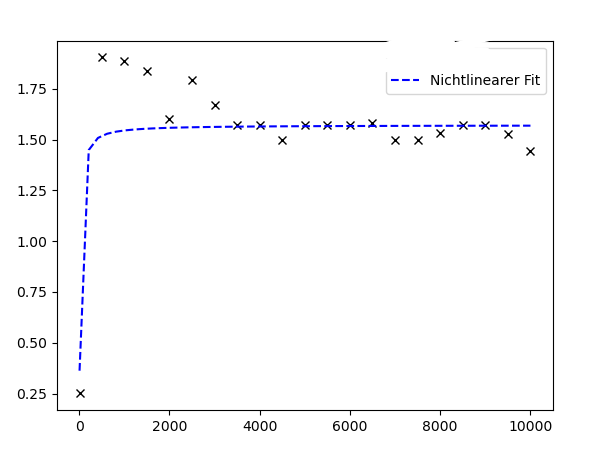
\includegraphics[width=0.9\textwidth]{build/plot1.pdf}
    \caption{Graphische Darstellung der annähernd linearen Werte aus der Messrehe der Wellenlänge $\protect \lambda = \SI{578}{\nano\meter}$ mit eingeszeichneter linearen Ausgleichsgerade. Dabei sind die Parameter $\protect a = \SI{-0.6043(390)}{}$ und $b = \SI{0.2417(231)}{}$.} 
    \label{fig:gelb}
\end{figure}

\begin{figure}
    \centering
    \includegraphics[width=0.9\textwidth]{build/plot2.pdf}
    \caption{Graphische Darstellung der annähernd linearen Werte aus der Messrehe der Wellenlänge $\protect \lambda = \SI{546}{\nano\meter}$ mit eingeszeichneter linearen Ausgleichsgerade. Dabei sind die Parameter $\protect a = \SI{-0.8503(457)}{}$ und $b = \SI{0.6500(240)}{}$.} 
    \label{fig:grün}
\end{figure}

\begin{figure}
    \centering
    \includegraphics[width=0.9\textwidth]{build/plot3.pdf}
    \caption{Graphische Darstellung der annähernd linearen Werte aus der Messrehe der Wellenlänge $\protect \lambda = \SI{435}{\nano\meter}$ mit eingeszeichneter linearen Ausgleichsgerade. Dabei sind die Parameter $\protect a = \SI{-0.6267(178)}{}$ und $b = \SI{0.7332(96)}{}$.} 
    \label{fig:violet}
\end{figure}

\begin{figure}
    \centering
    \includegraphics[width=0.9\textwidth]{build/plot4.pdf}
    \caption{Graphische Darstellung der annähernd linearen Werte aus der Messrehe der Wellenlänge $\protect \lambda = \SI{408}{\nano\meter}$ mit eingeszeichneter linearen Ausgleichsgerade. Dabei sind die Parameter $\protect a = \SI{-0.5892(331)}{}$ und $b = \SI{0.2042(196)}{}$.} 
    \label{fig:GIGAviolet}
\end{figure}
\newpage

\subsection{Bestimmung des Verhältnis von $\protect h$/$\protect e_{0}$}

Zur Bestimmung des Verhältnis der beiden Naturkonstanten $\protect h$/$\protect e_{0}$ werden die zuvor bestimmten Grenzspannungen in Abhängigkeit der verwendeten Frequenz des Lichts $\nu$ dargestellt.
Dieser Zusammenhang wird genau durch Gleichung \eqref{eq:imp} beschrieben. Die Messwerte haben also in der Theorie einen linearen Zusammenhang der sich auch in der Abbildung ... bestätigt.
\\
Wieder kann durch diese Messwerte eine lineare Ausgleichsgerade gelegt werden und die Parameter liefern Aufschluss auf das Verhältnis der Naturkonstanten $\protect h$/$\protect e_{0}$.
Zunächst kann die Gleichung \eqref{eq:imp} nach $U_{g}$ umgeformt werden und es ergibt sich
\begin{equation}
U_{g} = \frac{h}{e_{0}} \nu - \frac{W_A}{e_{0}}
\end{equation}
Ein Koeffizientenvergleich mit der allgemeinen Ausgleichsgeraden \eqref{eqn:okay} liefert die Parameter
\begin{align}
    \label{eq:1}
a &= \frac{h}{e_{0}},\\
    \label{eq:2}
b &= \frac{W_A}{e_{0}},
\end{align}
dabei gibt $a$ die Steigung der Geraden in [$\si{\joule\per\ampere}$] und $b$ die Austrittsarbeit in [$\si{\electronvolt}$] an.
Die Parameter ergeben sich wieder durch einen \enquote{Polyfit} erster Ordnung mit \enquote{Numpy} \cite{numpy} und den Relationen \eqref{eq:1} und \eqref{eq:2} zu
\begin{align}
\frac{h}{e_{0}} &= \SI{4.0132(13517)e-15}{\joule\per\ampere},\\
\frac{W_A}{e_{0}} &= \SI{-1.5722(7979)}{\electronvolt}.
\end{align}

Die Ausgleichsgerade sowie die Messwerte der Grenzspannungen sind in der Abbildung \ref{fig:3} dargestellt.

\begin{figure}
    \centering
    \includegraphics[width=0.9\textwidth]{build/plot5.pdf}
    \caption{Frequenzabhängige Grenzspannung mit linearer Ausgleichsgerade.}
    \label{fig:3}
\end{figure}

\subsection{Genauere Untersuchung und Deutung des Photostroms bei gelbem Licht.}

In dem Folgenden Diagramm \ref{fig:1} ist der Spannungsabhängige Photostrom zur Wellenlänge $\lambda = \SI{578}{\nano\meter}$ eingezeichnet. Desweiteren ist in der Abbildung \ref{fig:2} der Abschnitt bei Bremsspannungen, also $U > \SI{0}{\volt}$, nochmal einzeln dargestellt
da er in der Größenordnung des Gesamtbetrachtung untergeht.

\begin{figure}
    \centering
    \includegraphics[width=0.9\textwidth]{build/plot6.pdf}
    \caption{Spannungsabhängiger Photostom $\protect I$ bei einer Wellenlänge von $\protect \lambda = \SI{578}{\nano\meter}$.} 
    \label{fig:1}
\end{figure}

\begin{figure}
    \centering
    \includegraphics[width=0.9\textwidth]{build/plot7.pdf}
    \caption{Betrachtung der positiven Spannungswerte des Photostroms bei $\protect \lambda = \SI{578}{\nano\meter}$. } 
    \label{fig:2}
\end{figure}

Anhand dieser Abbildungen lassen sich nun folgende Dinge erläutern. 
\\
Bei hohen beschleunigenden Spannungen also für Spannungswerte $U << \SI{0}{\volt}$ erreicht die Kurve einen Sättigungswert an Photostrom, dies lässt sich folgendermaßen begründen. 
Die verwendete Lichtquelle besitzt bei der Wellenlänge $\lambda = \SI{578}{\nano\meter}$ eine feste Energie und durch die optischen Elemente bildet sich eine konstante Intensität des Lichts auf dem Eintrittsspalt zur Kathode aus. Das bedeutet also,
dass die Anzahl der Photonen pro Fläche und Zeit konstant ist und da jedes Photon maximal ein Elektron lösen kann gibt es einen Grenzfall. Bei beliebig großen beschleunigenden Spannungen werden irgendwann alle Elektronen an der Anode ankommen und diese entsprechen maximal der Anzahl der eintreffenden Photonen. Diese Grenze beschreibt
also das asymptotische Verhalten des Photostroms. Es können somit nicht mehr Elektronen gelöst werden als Photonen ankommen. Desweiteren wird der maximale Strom bei fester Energie des Lichts auch von der Anzahl der Valenzelektronen der Kathode festgelegt.
Der Strom näher sich dabei nur asymptotisch einem Grenzwert für hohe Spannungen auf Grund verschiedener Faktoren. Zum einen kommt es durch die Fermi-Energie zu unterschiedlichen Spannungen die nötig sind um ein Elektron zur Anode zu befördern, somit steigt der Strom zumindest nicht abrupt an. Außerdem spielt die mittlere freie
Weglänge der Elektronen in der Photozelle eine Rolle, da nicht von einem perfekten Vakuum ausgegangen werden kann. Eine möglichst hohe Spannung sorgt dafür, dass die Elektronen selbst nach Wechselwirkung mit den Atomen in der Luft noch an der Anode ankommen.
\\
Durch Temperaturen von knapp $\SI{20}{\celsius}$ also Raumtemperatur kann es bereits zu thermisch gelösten Elektronen an der Photokathode kommen, auf Grund der Bremspannung gehen diese zurück zur Kathode und es ist ein entgegengesetzter Strom messbar. Bei sehr hohen Temperaturen lässt sich
dieser Strom deutlich erhöhen. Der Sättigungswert ist also vor allem durch die Temperatur limitiert. Dieses Phänomen ist in Abbildung \ref{fig:2} erkennbar. Da bereits bei kleinen Lichtenergien ein negativer Strom auftritt lässt sich sagen, dass sich die Austrittsarbeit der Anode nicht sehr stark von der Austrittsarbeit der Kathode unterscheiden kann.
Vor allem kann sie nicht sehr viel größer sein, da $h\nu$ stets größer als $A_A$ sein muss, damit ein Strom messbar ist. Dadurch lässt sich die Austrittsarbeit der Anode $A_A$ auf 
\begin{equation}
A_A \leq \SI{1.908}{\electronvolt},
\end{equation}
bei einer Wellenlänge von $\lambda \approx \SI{650}{\nano\meter}$, abschätzen.